\documentclass[letterpaper]{article} % DO NOT CHANGE THIS
\usepackage[submission]{aaai2027}  % DO NOT CHANGE THIS
\usepackage[hyphens]{url}  % DO NOT CHANGE THIS
\usepackage{graphicx} % DO NOT CHANGE THIS
\urlstyle{rm} % DO NOT CHANGE THIS
\def\UrlFont{\rm}  % DO NOT CHANGE THIS
\usepackage{natbib}  % DO NOT CHANGE THIS AND DO NOT ADD ANY OPTIONS TO IT
\usepackage{caption} % DO NOT CHANGE THIS AND DO NOT ADD ANY OPTIONS TO IT
\frenchspacing  % DO NOT CHANGE THIS
\usepackage{amsmath}
\usepackage{amssymb}
\usepackage{amsthm}
\usepackage{booktabs}
\usepackage{array}
\usepackage[table]{xcolor}

\newtheorem{proposition}{Proposition}

\definecolor{pennblue}{HTML}{011F5B}
\definecolor{pennred}{HTML}{990000}
\definecolor{controlgray}{HTML}{444444}
\definecolor{pennbluefill}{HTML}{E8EEF5}
\definecolor{pennredfill}{HTML}{F7EAEA}
\definecolor{controlfill}{HTML}{F3F3F3}

\newcommand{\helpful}[1]{\textcolor{pennblue}{\bfseries #1}}
\newcommand{\utilityhelpful}[1]{\textcolor{pennblue}{\bfseries #1}}
\newcommand{\harmful}[1]{\textcolor{pennred}{\bfseries #1}}
\newcommand{\neutral}[1]{\textcolor{controlgray}{#1}}
\newcommand{\diagnostic}[1]{\textcolor{controlgray}{#1}}

\pdfinfo{
/TemplateVersion (2027.1)
}

\title{Fixed-Spectrum Swaps Separate Attention Capacity from Assignment}
\author{Anonymous Submission}
\affiliations{}

\begin{document}
\setcounter{secnumdepth}{2}
\maketitle

\begin{abstract}
Attention concentration cannot identify where a transformer routes information: two attention rows may share
the same weight spectrum while assigning their largest weights to different tokens. We introduce
fixed-spectrum swaps, a causal intervention that preserves every permutation-invariant property of an attention
row while changing its assignment to task-labeled positions. Across controlled retrieval, pretrained language
models, and context-grounded question answering, the intervention separates selective capacity from correct
assignment and reveals assignment-responsive, saturated, and selector-mismatch regimes. A local value-aware
utility term ranks finite margin effects in controlled retrieval with $0.989$ Spearman correlation and $99.5\%$
sign agreement, and utility-selected circuits yield positive held-out effects on natural question answering.
Context-length sweeps stress-test these diagnoses and identify cases where routing changes do not account for
behavioral degradation. Fixed-spectrum swaps provide a controlled test of whether attention assignment causally
affects a model's prediction.
\end{abstract}

\section{Background}

Our question is whether attention concentration identifies task-correct routing. \emph{At fixed concentration,
does assigning the same attention spectrum to task-required evidence change the prediction?}

Length degradation motivates this question. A transformer may learn a retrieval rule on short sequences and
then lose it as distractors accumulate. We see this pattern in copying, key--value recall, and algorithmic tasks
\citep{kazemnejad,nopeentropy,sparselong}. As contexts grow, attention often becomes more diffuse, entropy rises,
and attention-output variance can collapse \citep{vanishingvariance}. These trends describe scale and
concentration, yet they do not tell us where the attention goes.

The non-identifiability is structural. Two attention rows can share their sorted weights, entropy, maximum, and
every norm while placing their largest weights on different tokens. One can favor the evidence and the other a
distractor.

We answer with a fixed-spectrum intervention. At the answer query, we exchange the weight on a known source
with a distractor weight and then run the unchanged model. Because the exchange preserves the complete
spectrum, a distractor-only exchange gives a matched control. This paired setup brings a second question into
focus: when does moving weight to the source help? The answer depends on the spectrum's selective capacity,
its assignment to task-labeled positions, and the downstream utility of the moved values.

The controlled result is clear. Source-max raises per-token accuracy by $0.153$, source-min lowers it by
$0.043$, and the distractor control changes it by $0.011$. As the spectrum sharpens, the gap between the two
assignments grows even though sharpening the original assignment remains near zero. A local utility term then
orders the finite margin effect with $0.989$ Spearman correlation and $99.5\%$ sign agreement. The same
direction appears in Qwen and Pythia, while Gemma and SmolLM2 reveal saturation and selector mismatch.
Utility-selected routing also transfers to context-grounded natural QA.

Our contributions are:
\begin{itemize}
    \item \textbf{Fixed-spectrum identification.} We separate selective capacity from task-conditioned
    assignment by preserving the complete attention spectrum and altering only its token placement.
    \item \textbf{Utility-conditioned mechanism.} We characterize when source--donor reassignment changes
    the final output and test the prediction against exact interventions.
    \item \textbf{Transfer and boundaries.} We test the intervention across controlled tasks, pretrained models,
    multi-evidence computation, and natural QA, and identify saturation and selector-mismatch regimes.
\end{itemize}

\begin{figure*}[!t]
\centering
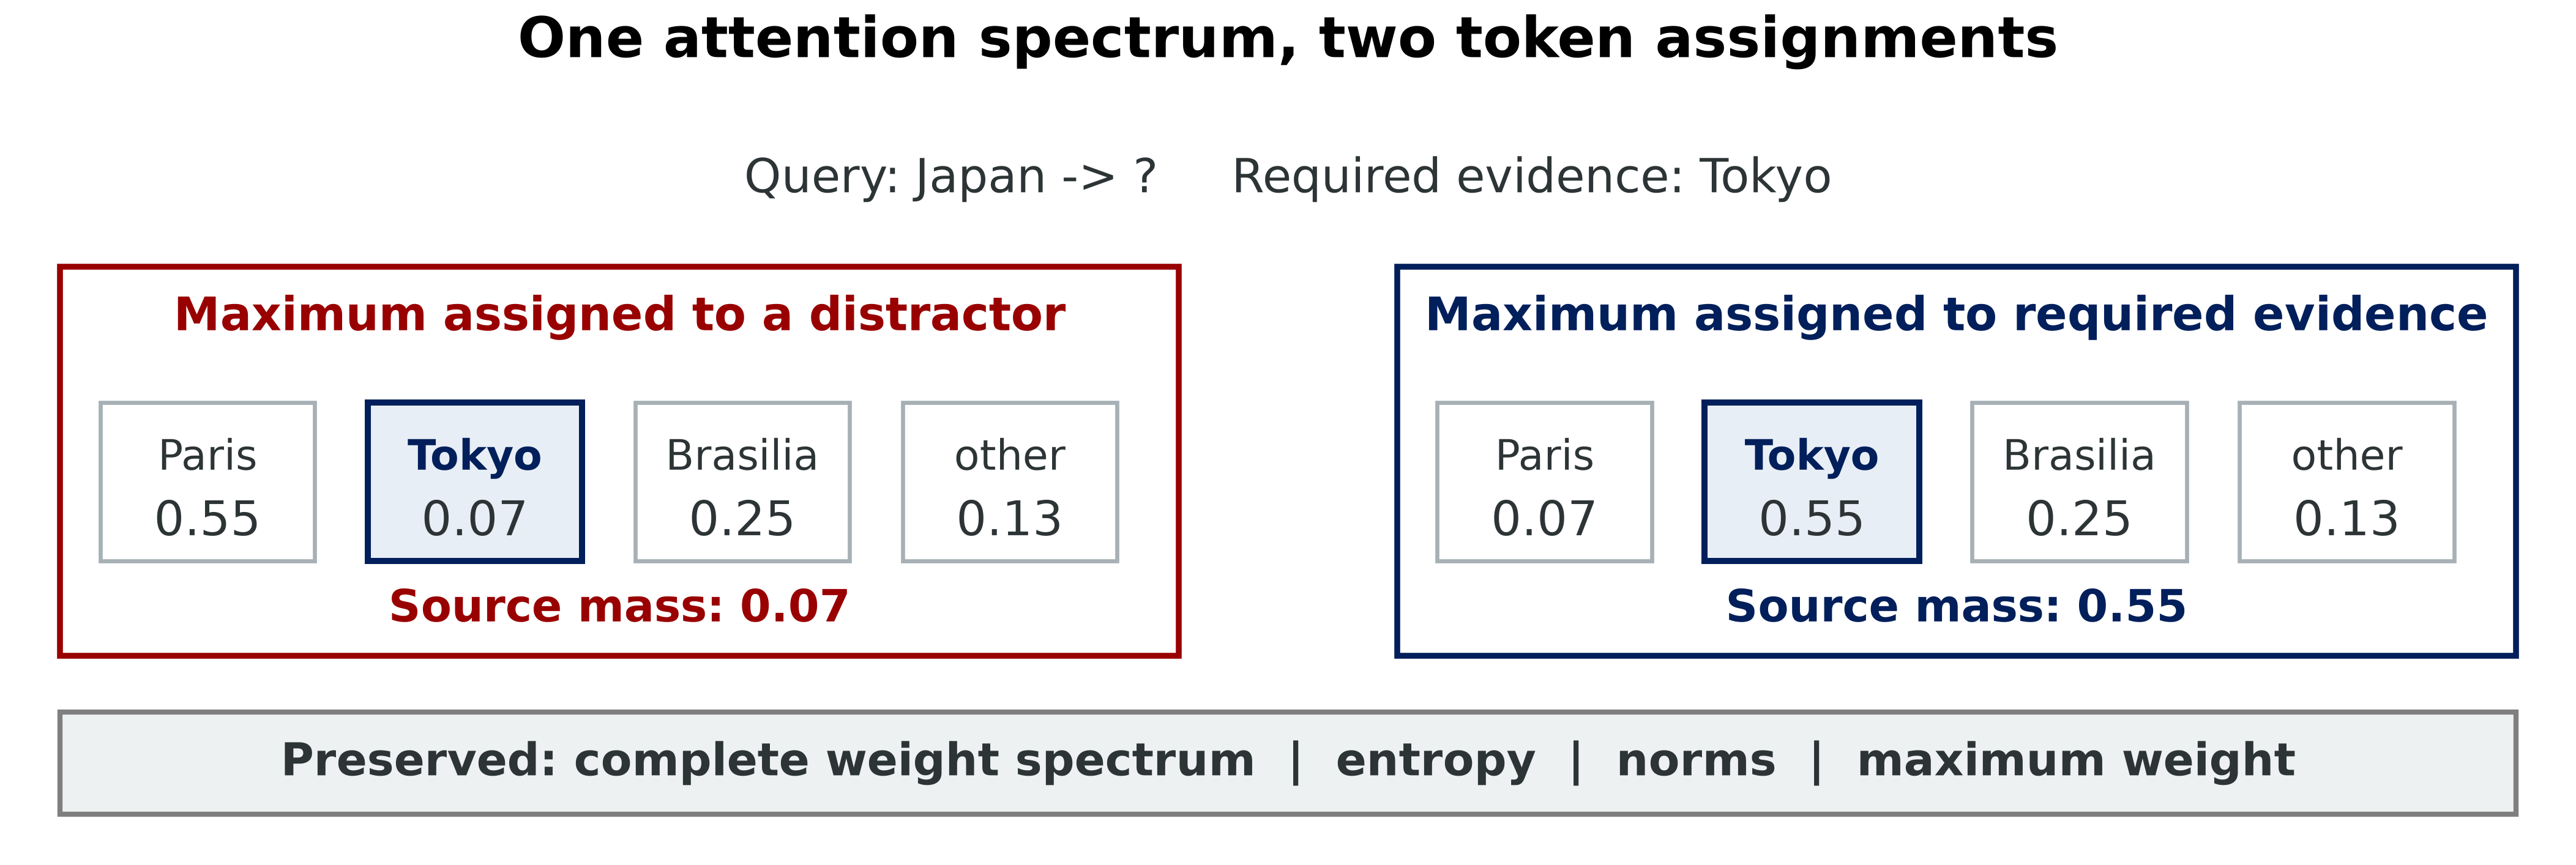
\includegraphics[width=0.97\textwidth]{figures/fig_routing_overview.png}
\caption{Fixed-spectrum reassignment changes destination while preserving concentration. The same
four weights place the maximum on a distractor (left) or the required evidence (right). Output behavior can
change only through the moved values and the downstream circuit that reads them.}
\label{fig:overview}
\end{figure*}

\section{Related Work}

\paragraph{Attention concentration and what it does not identify.}
Attention concentration has been connected to optimization, token selection, extrapolation, and sparse
long-context computation \citep{maxmarginselection,nopeentropy,ssmax,sparselong}. Other accounts emphasize
attention-output scale or normalization \citep{vanishingvariance,postnorm}. These statistics often move
together as context length changes. They are used as evidence in routing accounts, but their status as
identifying measures of task-correct routing is generally untested. Our intervention tests that identification
question while the entire spectrum is held fixed.

\paragraph{Attention intervention and non-identifiability.}
Attention weights have long been studied as explanations, perturbed to test prediction sensitivity, and
shown to be non-identifiable without their value vectors
\citep{jainwallace2019,wiegreffepinter2019,brunner2020identifiability,kobayashi2020weight,hassid2022papa}.
Causal circuit analysis takes the next step by patching internal activations and measuring the output change
\citep{yamakoshi2023causal,conmy2023acdc}. Attribution patching uses a gradient approximation to screen many
candidate components efficiently \citep{syed2023attribution,kramar2024atp}. Our utility term has a related
first-order form. Here we evaluate it along an exact permutation of a model's own attention row, alongside the
finite swap itself.

\paragraph{Closest attention interventions.}
Attention Knockout blocks selected edges and renormalizes the row to trace factual information flow
\citep{geva2023dissecting}. Efficient attention projects a row onto its output-effective subspace and studies
when attention supports causal explanation \citep{naim2024explaining}. Contribution Weights combine attention
mass with projected-value magnitude and alignment, then test token importance through removal
\citep{cunningham2026contribution}. These approaches delete, block, renormalize, or rank parts of an attention
pathway. Our reassignment leaves the complete attention-weight multiset intact and changes its assignment to
token positions. Equation~\ref{eq:margin-bound} then connects that finite, task-labeled swap to the target margin.

\paragraph{Retrieval-based long-context architectures.}
Sparse and retrieval-based architectures ask how a model can access distant context efficiently
\citep{sparselong,hu2025causalretrieval}. Grouped Cross Attention, for example, learns to retrieve useful
chunks into a bounded attention window. We study a different object: a trained attention row with a fixed
weight spectrum. The goal is to isolate the behavioral effect of assigning its available selectivity to
task-required evidence.

\section{Methods}

\subsection{Capacity and Assignment}

At an answer query, let $a=(a_1,\ldots,a_n)$ be an attention row over $n$ token positions, where $a_j\ge0$
and $\sum_j a_j=1$. Let $S\subseteq\{1,\ldots,n\}$ contain the $r=|S|$ task-required evidence positions,
and let $a_{(1)}\ge\cdots\ge a_{(n)}$ denote the same weights in descending order. Define
\begin{equation}
\begin{aligned}
 C_r^+&=\sum_{i=1}^{r}a_{(i)}, &
 C_r^-&=\sum_{i=n-r+1}^{n}a_{(i)},\\
 K_r(a)&=C_r^+-C_r^-.
\end{aligned}
\label{eq:capacity}
\end{equation}
$C_r^+$ and $C_r^-$ are the largest and smallest evidence masses available under permutations of the fixed
spectrum, and $K_r(a)$ is the available routing range. An assignment is a permutation $\pi$ of
$\{1,\ldots,n\}$ that places weight $a_{\pi(j)}$ at token position $j$. Its evidence mass and normalized
assignment coordinate are
\begin{equation}
\begin{aligned}
 m_S(\pi)&=\sum_{j\in S}a_{\pi(j)},\\
 \rho_S(\pi)&=\frac{m_S(\pi)-C_r^-}{K_r(a)}\in[0,1],\qquad K_r(a)>0.
\end{aligned}
\label{eq:assignment-coordinate}
\end{equation}
Thus $m_S(\pi)=C_r^-+\rho_S(\pi)K_r(a)$. If $K_r(a)=0$, every assignment has the same evidence mass.

\begin{center}
\fcolorbox{pennblue}{pennbluefill}{\parbox{0.92\columnwidth}{
\textbf{Capacity} specifies how much evidence mass the spectrum can support.\\
\textbf{Assignment} specifies where that mass is placed.\\
\textbf{Utility} specifies whether moving it changes the answer.
}}
\end{center}

\begin{proposition}[Fixed-spectrum capacity--assignment decomposition]
For every assignment $\pi$ of a fixed weight multiset,
\begin{equation}
 C_r^-\le m_S(\pi)\le C_r^+,
\end{equation}
and both bounds are attained. If $K_r(a)>0$, Equation~\ref{eq:assignment-coordinate} defines a unique
$\rho_S(\pi)$. No statistic invariant to token permutation can determine $\rho_S$.
\label{prop:capacity}
\end{proposition}

\paragraph{Proof sketch.}
An $r$-position evidence set receives at most the $r$ largest weights and at least the $r$ smallest. Assigning
those weights to $S$ attains each endpoint. Normalizing evidence mass within this interval gives $\rho_S$.
Any permutation-invariant statistic is constant across all assignments, including assignments at opposite
endpoints. The supplement gives the full exchange argument and the corresponding affine margin range.
The decomposition is algebraic for every $r$. Behavioral validation is positive for $r=1$ and $r=2$; the
$r=3$ interval includes zero and the $r=4$ models miss competence, so efficacy at higher arity is unestablished.

\subsection{Utility-Conditioned Output Effects}

Capacity and assignment describe attention mass. Prediction also depends on values and downstream
computation. Let $H$ be the selected attention heads. In each $h\in H$, let $s$ be the evidence position,
$d_h$ the donor position whose weight is exchanged with it, and $a_{hj}$ the original attention weight on
position $j$. Define the transferred mass $\delta_h=a_{h d_h}-a_{h s}$. Let $x_{hj}$ be token $j$'s
residual-stream contribution after head $h$'s value and output projections. If $z$ is the unpatched residual
state, the intervention gives $z'=z+\Delta z$, where
\begin{equation}
 \Delta z=\sum_{h\in H}\delta_h(x_{hs}-x_{hd_h}).
\label{eq:residual-change}
\end{equation}
Let $\ell_k(z)$ be the downstream logit for token $k$, with target $y$ and competitor $c$. Define
$M_c(z)=\ell_y(z)-\ell_c(z)$, the exact change $\Delta M_c=M_c(z+\Delta z)-M_c(z)$, and local utility
$u_{hj}^{(c)}=\nabla_z M_c(z)^\top x_{hj}$.

\begin{proposition}[Utility-conditioned swap effect]
If $\nabla_z M_c$ is $L_c$-Lipschitz on $\{z+t\Delta z:t\in[0,1]\}$, then
\begin{equation}
 \Delta M_c=
 \sum_{h\in H}\delta_h\big(u_{hs}^{(c)}-u_{hd_h}^{(c)}\big)+R,
 \qquad |R|\le\frac{L_c}{2}\lVert\Delta z\rVert_2^2.
\label{eq:margin-bound}
\end{equation}
For an affine downstream margin, $R=0$.
\label{prop:utility}
\end{proposition}

The Taylor remainder is standard. Our contribution is the task-labeled capacity--assignment coordinate and
its coupling to the exact fixed-spectrum swap vector in Equation~\ref{eq:residual-change}.

The intervention transfers attention mass from a donor token to the source. It helps when the source
contributes more positively to the target margin than the displaced donor, unless downstream curvature
overwhelms that gain. Source-max can therefore succeed, saturate, or fail under the same attention-mass rule.
The supplement derives Equation~\ref{eq:margin-bound}, extends it to evidence sets, and states a sufficient
margin certificate.

\section{Experimental Setup}

\paragraph{Controlled tasks.}
Argmax retrieval presents key--value pairs and requests the value paired with the largest key. Flag retrieval
presents values with exactly one marked position and requests that value. Both have one labeled source.
Two-evidence modular sum marks two digits and requests their sum modulo ten, so both sources are required.
Four-layer decoders are trained with NoPE and RoPE and four seeds per cell; evaluation reaches $50\times$
training length. An eight-layer, width-$512$ grid checks scale. The inverse temperature $\beta\in\{1,2,4\}$
changes attention capacity while each assignment comparison preserves the resulting sorted spectrum.

\paragraph{Pretrained and natural-language tasks.}
In-context key--value recall lists pairs followed by a query key; the paired value is the labeled source.
We test Qwen2.5, Pythia, Gemma, and SmolLM2 across increasing pair counts. The selector audit compares circuits
ranked on disjoint calibration data by source mass or by output-conditioned utility. Natural MCQA uses
four-choice questions with one gold passage and unrelated passages. Questions must be correct with the full
context and gold passage alone, but incorrect without context. This filtering defines a model-specific
context-dependent subset and is not intended to estimate average performance over the full dataset. Its length
ladder freezes the four-passage circuit before forming nested 8-, 16-, and 32-passage contexts with additional
unrelated passages.

\paragraph{Interventions and estimation.}
The distractor control swaps the largest and smallest non-source weights, preserving source mass while
permuting the same attention row. For a source position $s$, let $d^+=\arg\max_j a_j$,
$d^-=\arg\min_j a_j$, and $D=\{j:j\ne s\}$ over valid tokens. Source-max swaps $(s,d^+)$ and source-min
swaps $(s,d^-)$. In controlled and pretrained key--value recall, the distractor control uses the maximum and
minimum within $D$. Natural QA uses a displacement-matched control. With
$\delta=a_{d^+}-a_s$, it chooses
\begin{equation}
 (p,q)=\arg\min_{\{j,k\}\subset D}
 \big\vert\,|a_j-a_k|-\delta\,\big\vert
 \label{eq:matched-control}
\end{equation}
and swaps $(p,q)$. Among all non-source pairs, this choice minimizes the absolute difference between the
control's $L_1$ displacement and the treatment's $L_1$ displacement; the remaining difference is the minimum
attainable mismatch for that row. It holds source mass fixed, and every control preserves the complete spectrum.
The natural control matches displacement first because it is the perturbation magnitude. It does not match the
donor token, positional distance, or value norm, which remain separate confounds. Calibration and
evaluation examples are disjoint, circuits are frozen before paired evaluation, and hierarchical intervals
resample calibration or model seeds above paired examples. We interpret a cell only after its frozen
competence gate passes.
Three confirmatory contrasts form one inferential family: controlled source-max versus distractor control,
the capacity-by-assignment interaction, and natural utility-selected source-max versus matched control. We use
two-sided exact sign-flip tests at the trained-model or calibration-seed cluster level and Holm correction across
the family. Other intervals are descriptive and unadjusted.
These swaps are counterfactual probes and need not lie on the model's endogenous query--key manifold. Treatment
and control share this intervention class, so their contrast measures downstream sensitivity to assignment,
rather than the frequency with which the model naturally creates a particular row. Layer controls ($+1.107$ for
selected $K=8$ versus $-0.059$ for a random layer) and coverage dose response show greater sensitivity under this
probe. They do not show that normal query--key computation produces swapped rows or that selected heads are the
exclusive retrieval mechanism. In untouched distractor-order variants, the conditional source-mass coefficient
is $+1.250$ ($p=.03125$), while the closest-spectrum paired effect is $+.026$ ($[-.017,+.070]$, $p=.25$).
This connects the intervention to an endogenous association without establishing endogenous causality.

\begin{figure}[!ht]
\centering
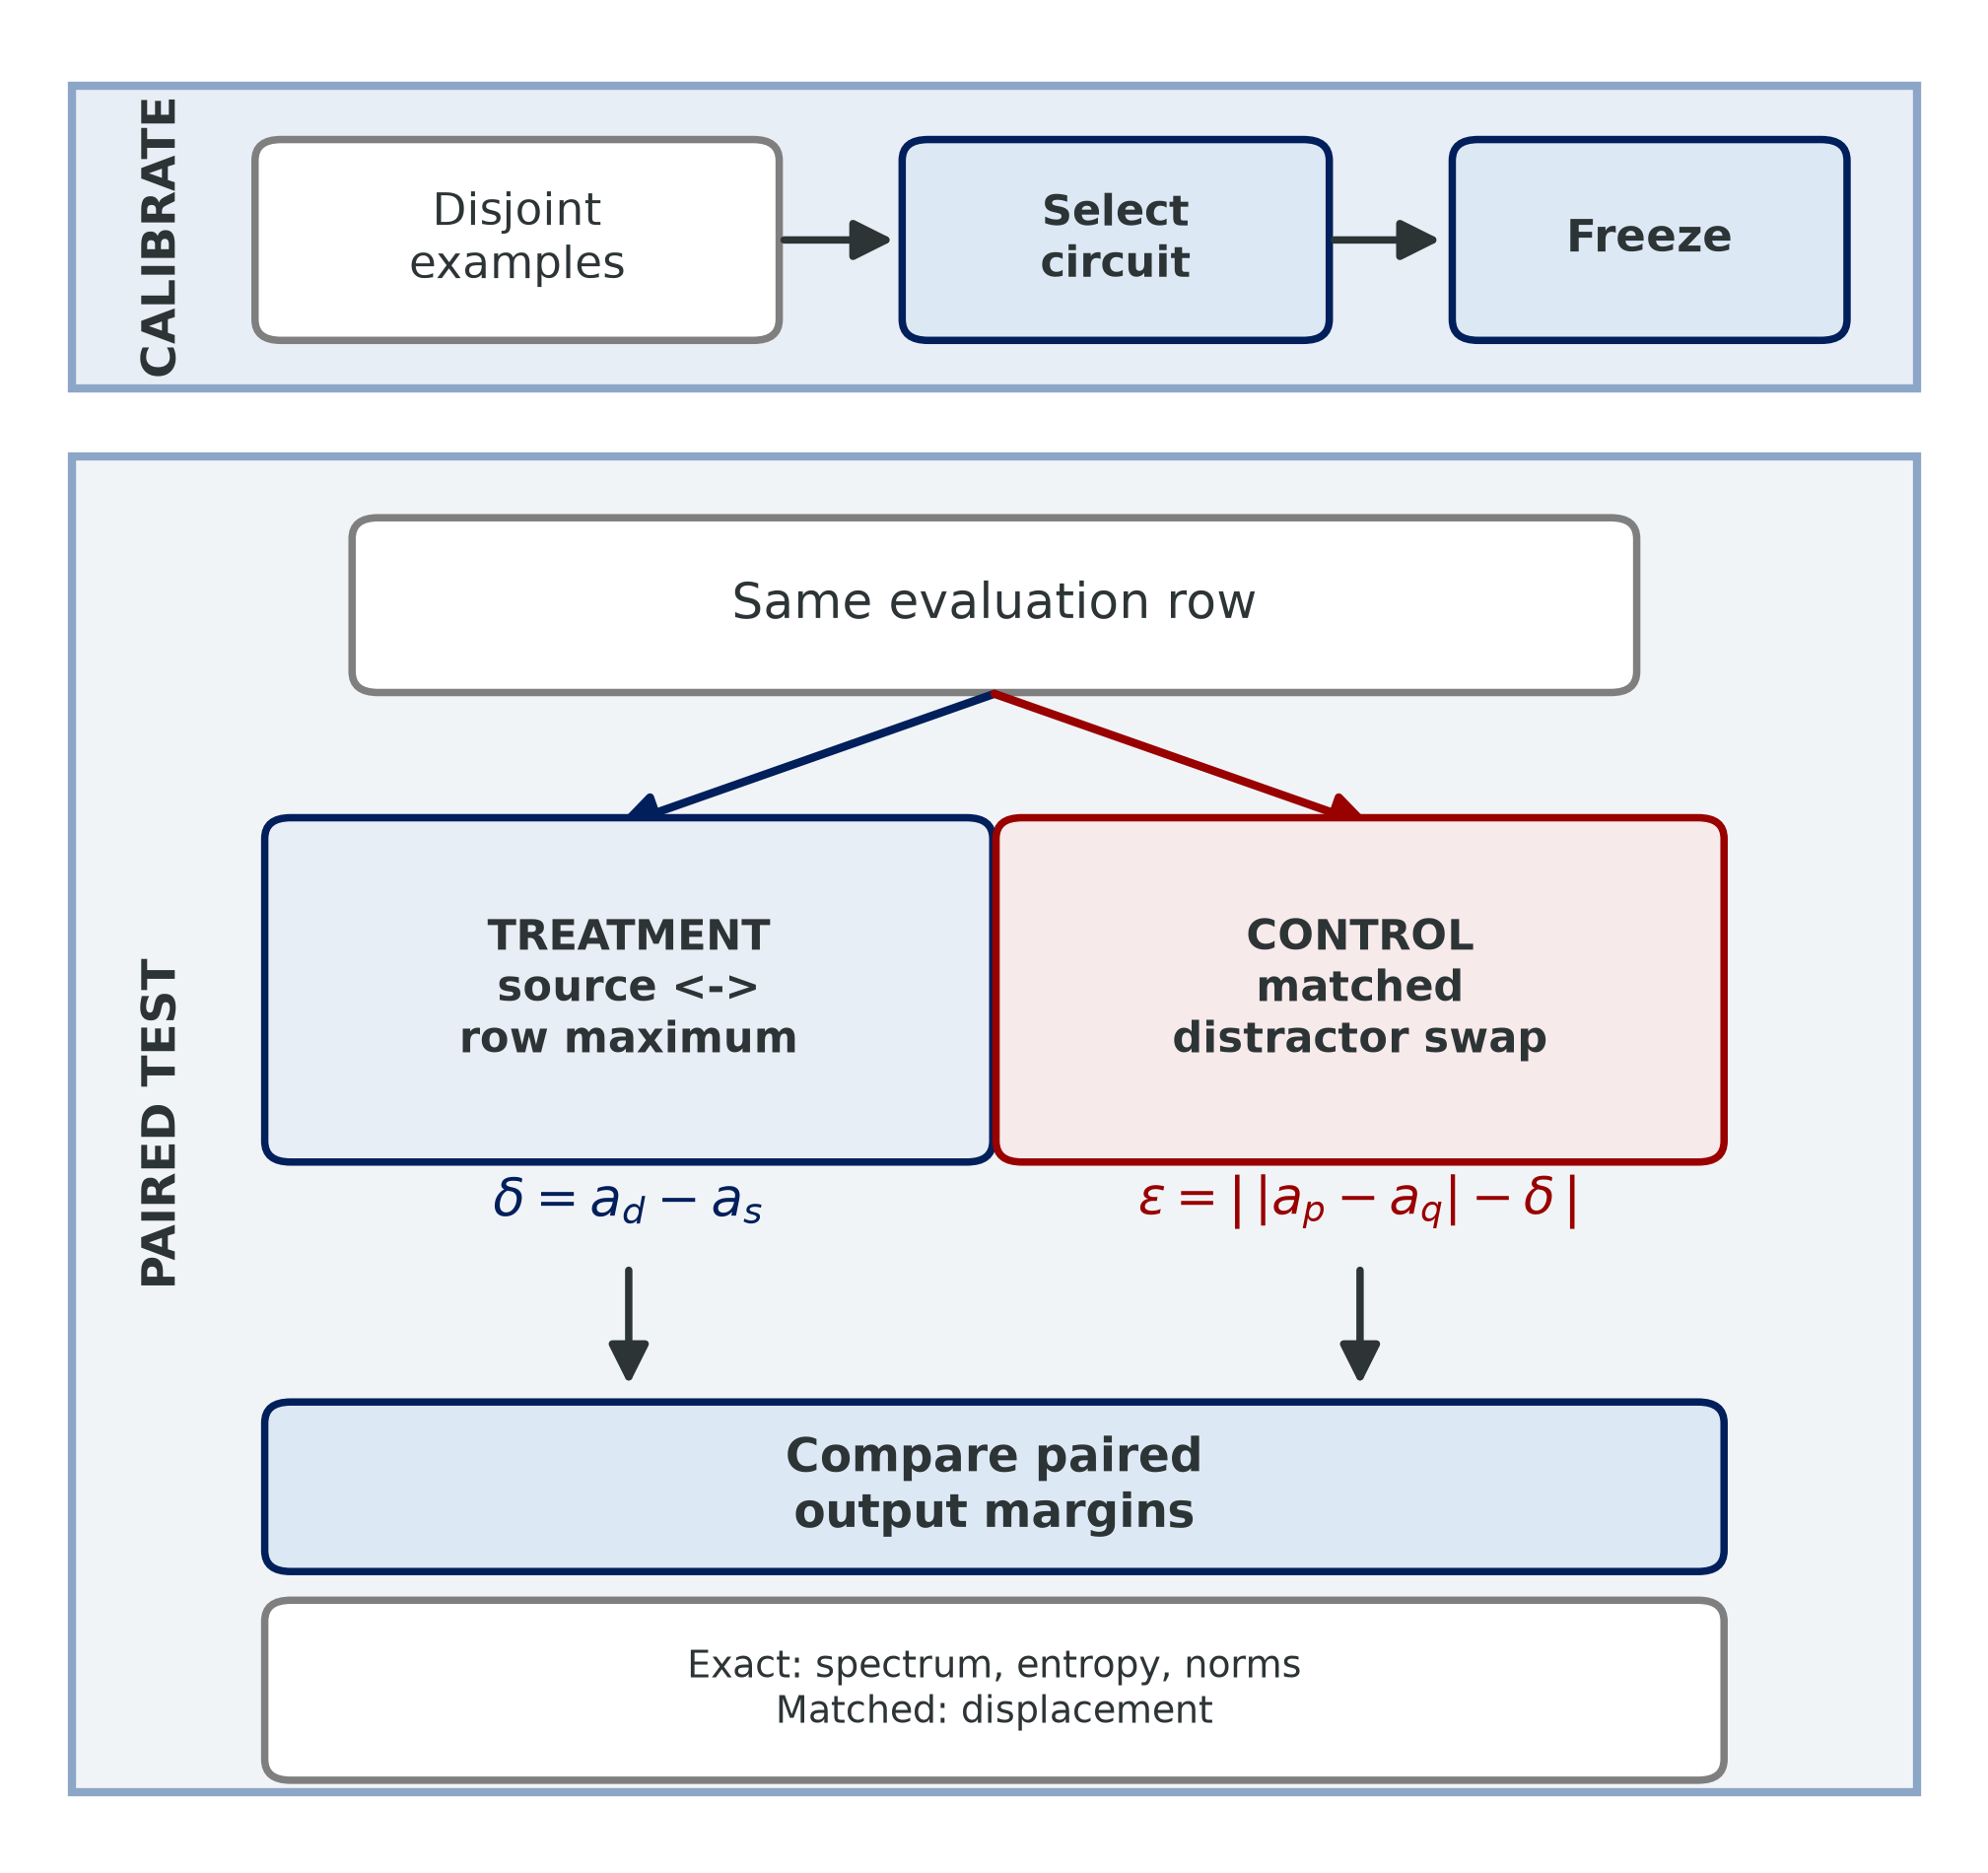
\includegraphics[width=0.96\columnwidth]{figures/fig_paired_causal_protocol.png}
\caption{Paired causal protocol. A circuit selected on disjoint calibration data is frozen before
treatment and control are applied to the same evaluation row. Both paths preserve the spectrum; the natural
QA control additionally minimizes displacement mismatch in Equation~\ref{eq:matched-control}.}
\label{fig:paired-protocol}
\end{figure}

\paragraph{Measured outcomes.}
We record task accuracy, target-versus-competitor margin, source mass, attention-output variance, entropy,
norms, and the full sorted spectrum. Every fixed-spectrum condition preserves the selected attention rows to
numerical precision. The supplement reports prompts, hyperparameters, per-length tables, competence failures,
and preregistered decision rules.

\section{Results and Discussion}

\subsection{Assignment Changes Accuracy at Fixed Spectrum}

\begin{figure*}[!t]
\centering
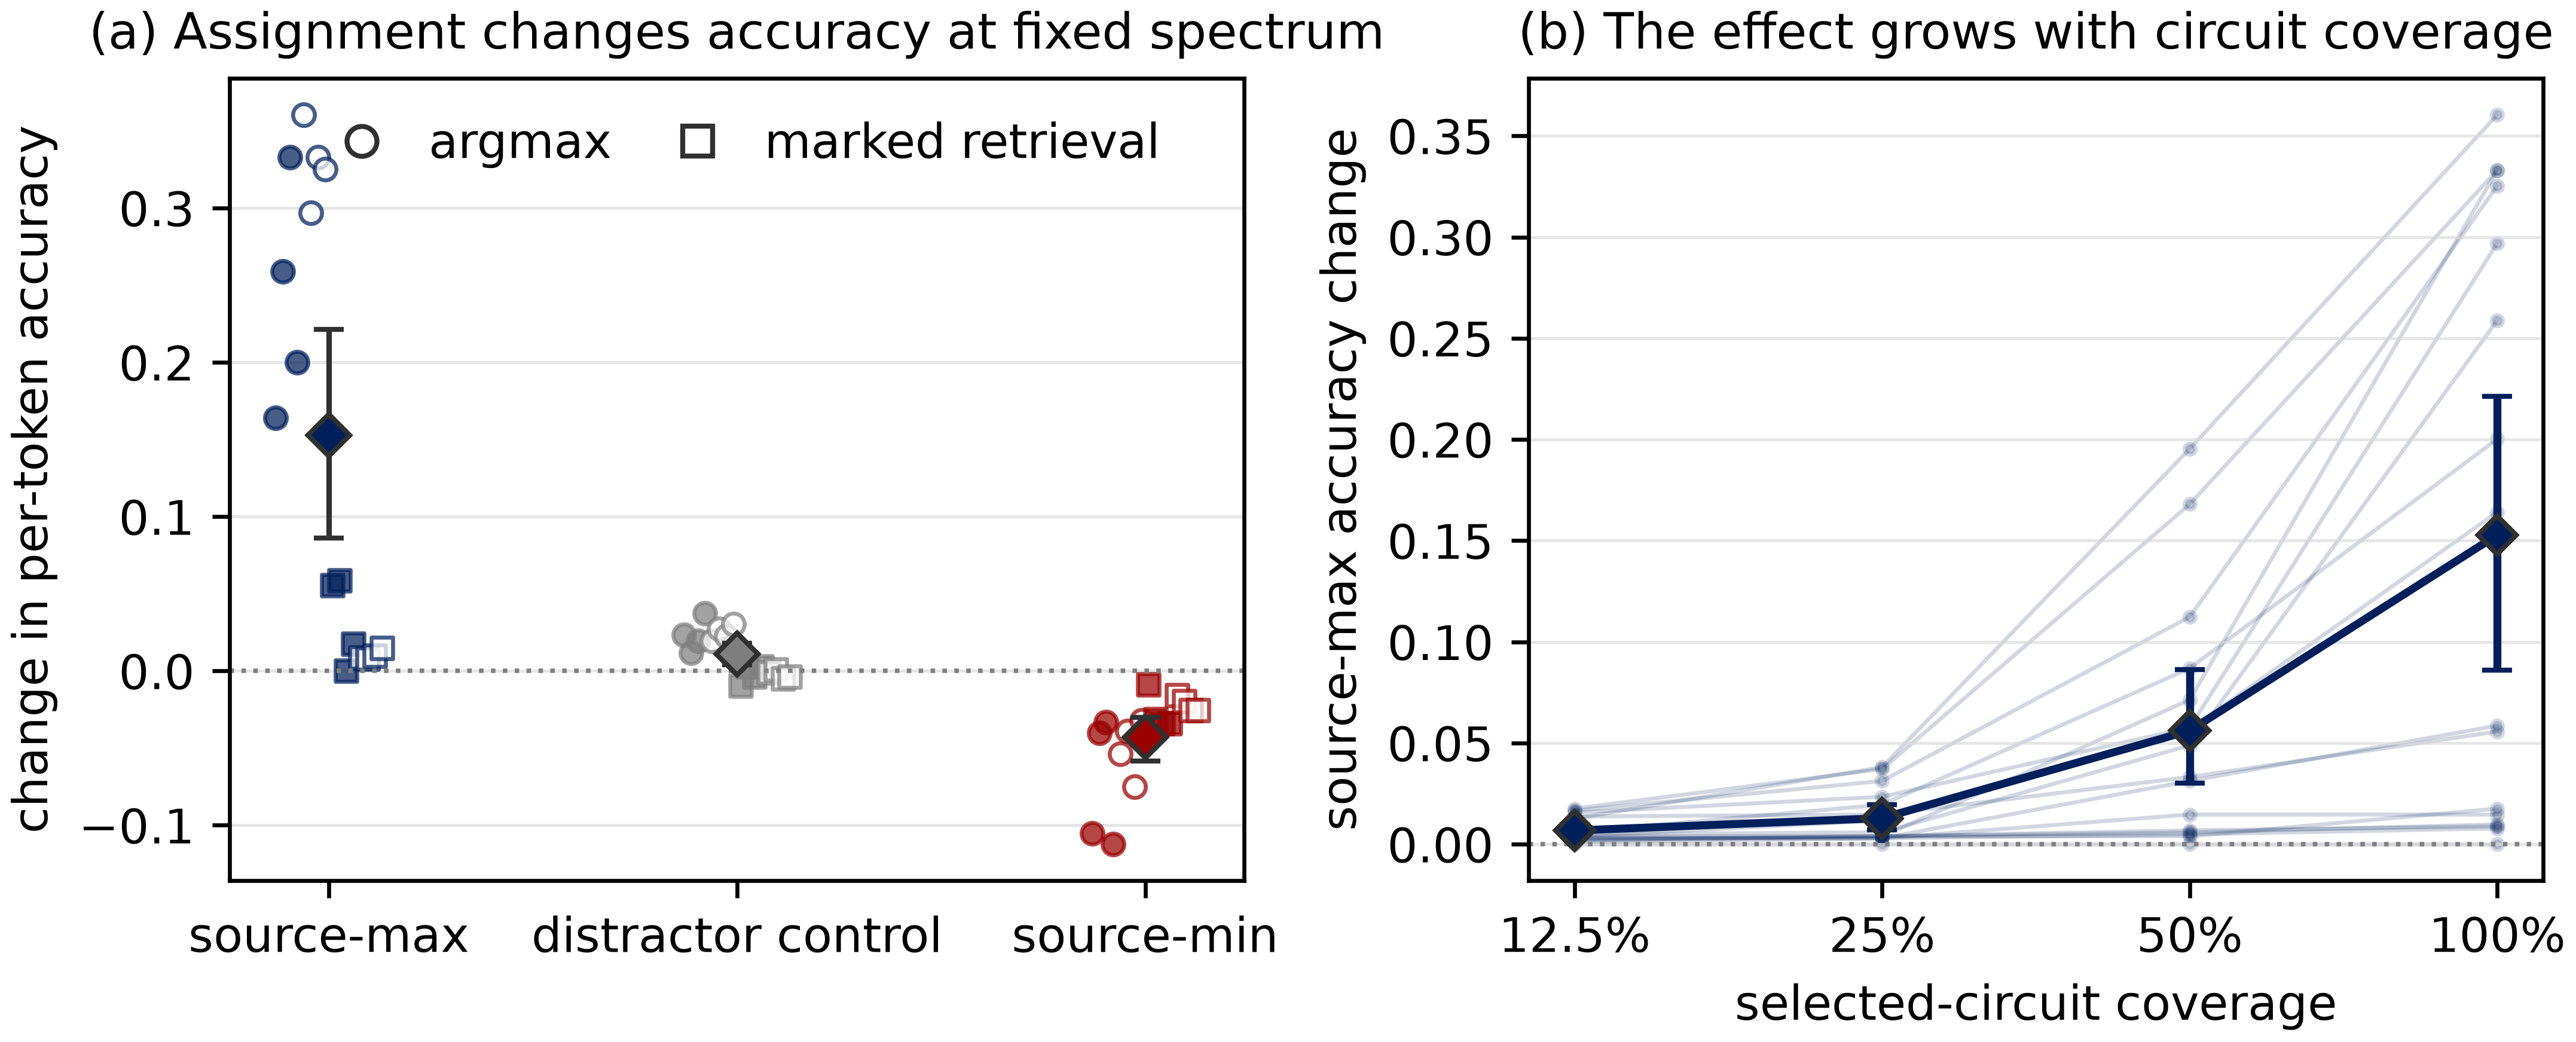
\includegraphics[width=0.88\textwidth]{figures/fig_fixed_spectrum_result.png}
\caption{Assignment changes retrieval despite an identical attention spectrum. Source-max improves accuracy,
source-min harms it, and the distractor-only control remains near zero (a). The effect increases with the
fraction of the selected circuit receiving the intervention (b). Diamonds and intervals summarize trained
models; faint paths show individual cells.}
\label{fig:assignment-effect}
\end{figure*}

We begin with the simplest test: move the largest available weight to the source, move it away, or exchange
two distractors. Across sixteen trained models, the mean changes are $+0.153$, $-0.043$, and $+0.011$,
respectively (Figure~\ref{fig:assignment-effect}). Source-max beats the control in every model--length
comparison. Their primary cluster-level contrast is $+.142$ (95\% CI $[+.080,+.206]$; exact
$p=3.05\times10^{-5}$; Holm-adjusted $p=9.16\times10^{-5}$), while complete-spectrum invariant error stays
below $10^{-6}$.

The controlled audit contains 8,192 head--example pairs. Individual swaps are vacuous in 18.5\% of them, but
only 86 of 1,024 complete eight-head circuits (8.4\%) are entirely vacuous. Mean exact margin change is $+3.891$
over all circuits and $+4.248$ (95\% CI $[+3.863,+4.640]$) over the 938 active circuits. The median per-head
transferred mass is $.025$ (90th percentile $.930$), and effect size rises across transfer quartiles. The
supplementary displacement audit reports the full distribution.

The effect grows with circuit coverage (Figure~\ref{fig:assignment-effect}b). Patching one, two, four, and eight
selected heads gives mean source-max gains of $0.007$, $0.013$, $0.056$, and $0.153$ and is monotone in 31 of
32 model--length comparisons, consistent with a distributed effect under the probe.

Source attention tracks accuracy more closely than attention-output variance. Normalizing that variance leaves
accuracy unchanged, whereas forcing mass onto the known source restores controlled retrieval. Sharpening the
original row has little effect.

The ordering survives the eight-layer replication, both positional encodings, four training seeds, and two
controlled tasks. Random-layer and adjacent-layer interventions remain near zero when the selected circuit is
held fixed. Full model-level intervals and the variance and patching results appear in the supplement.

\subsection{Capacity Amplifies Assignment}

\begin{figure*}[!t]
\centering
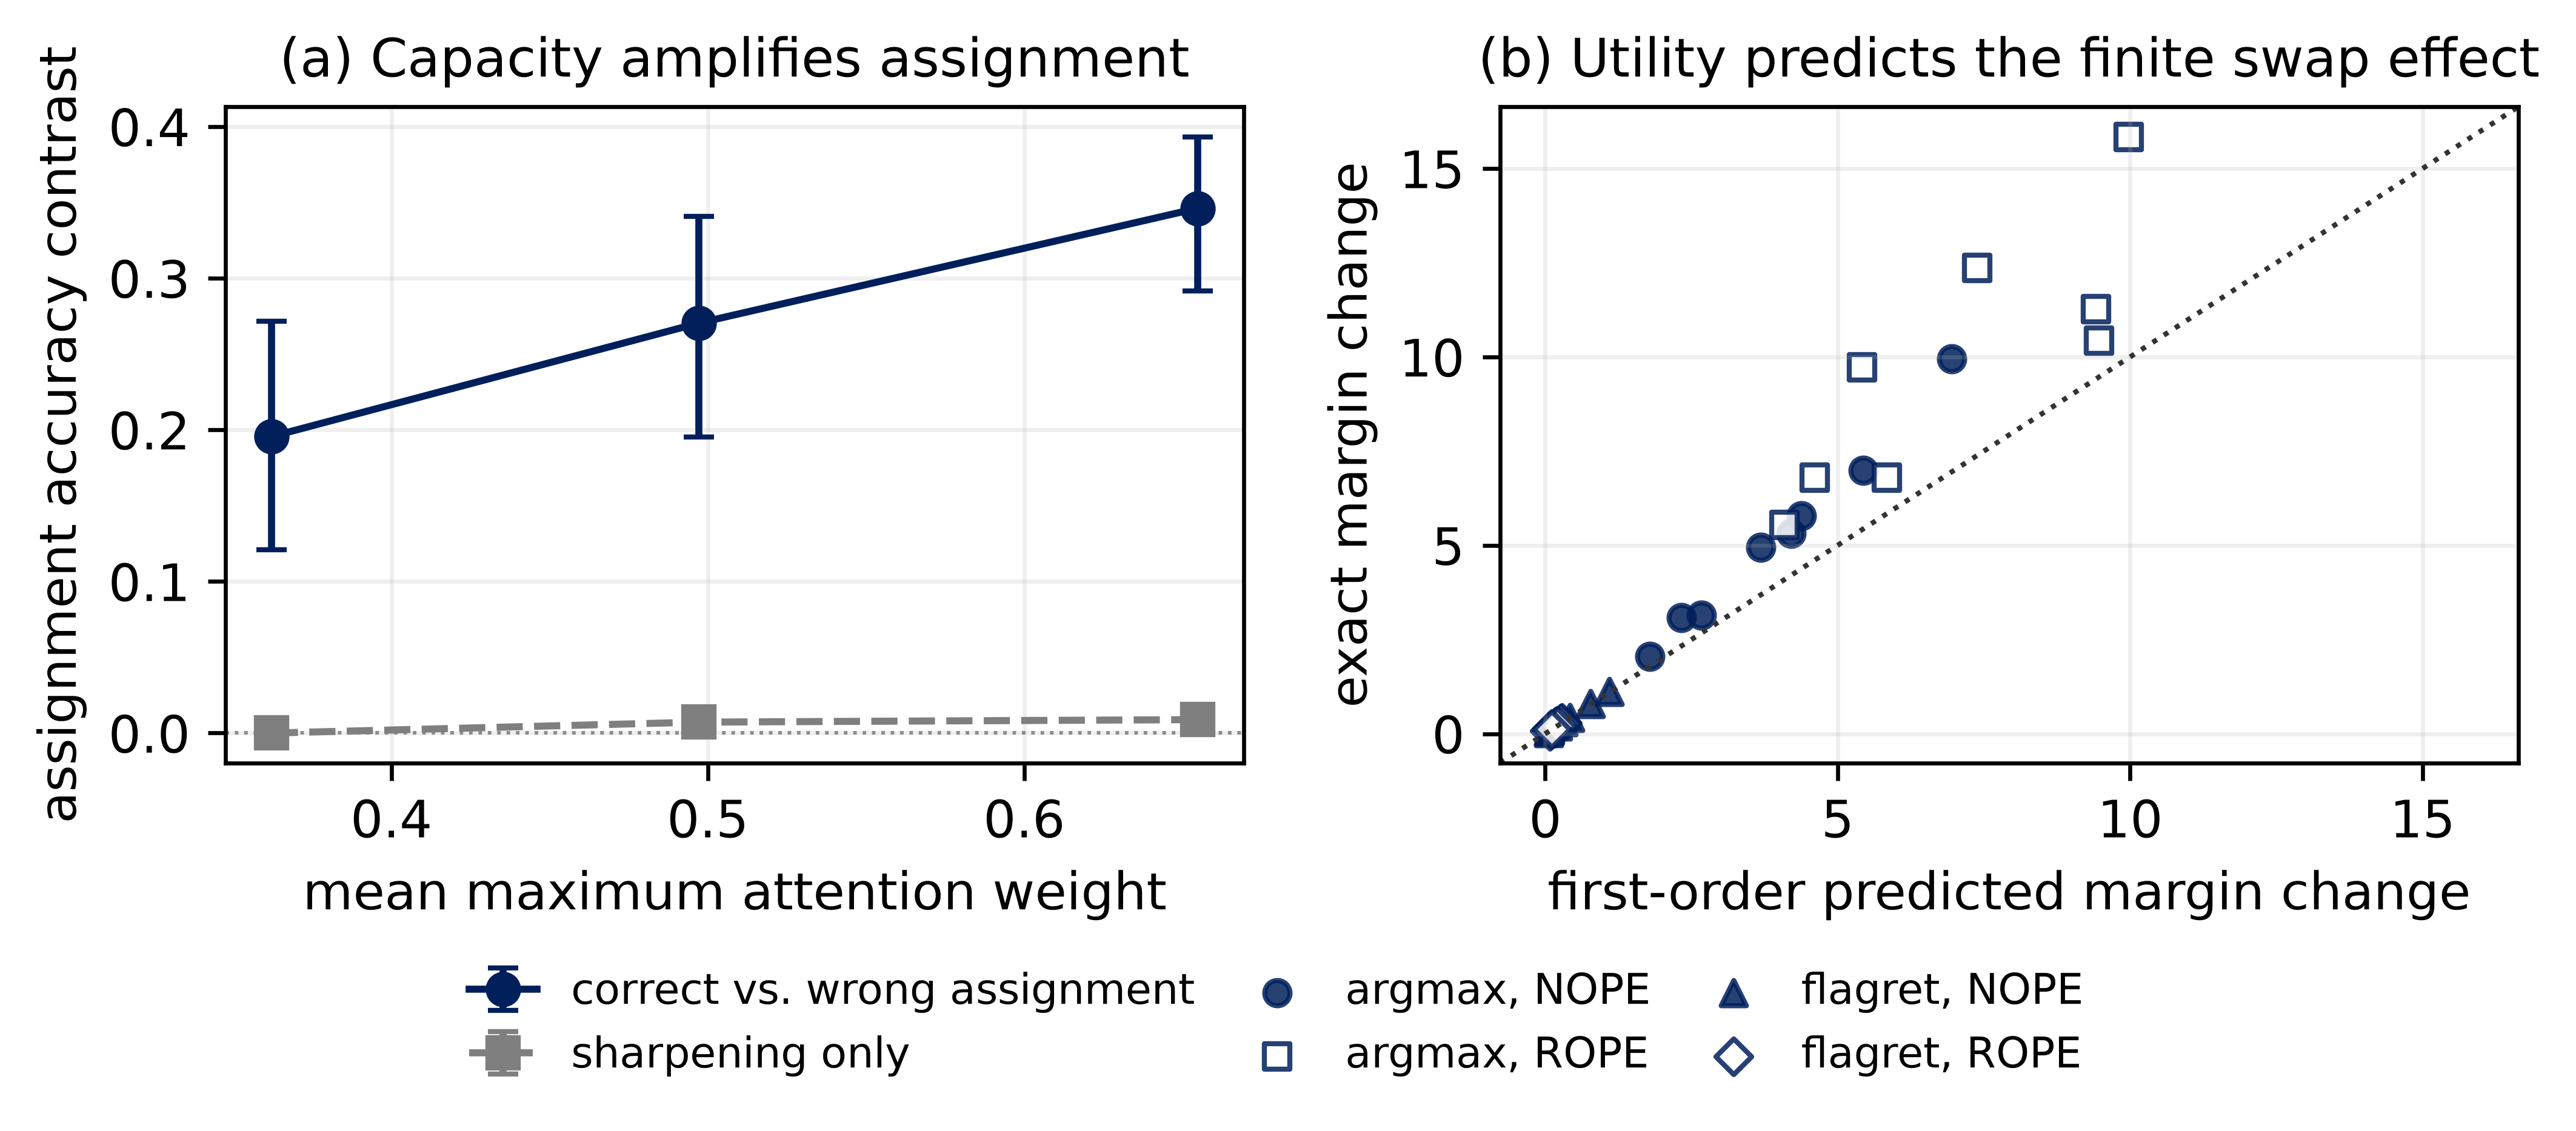
\includegraphics[width=0.84\textwidth]{figures/fig_capacity_assignment.png}
\caption{Capacity controls leverage, and utility predicts the finite intervention. Sharper spectra
increase the correct-versus-wrong assignment contrast while sharpening alone remains near zero (a). The
first-order utility term predicts the exact source-max margin effect across tasks and positional encodings
(b). Error bars summarize trained models.}
\label{fig:capacity-assignment}
\end{figure*}

We next vary spectrum and assignment independently. Temperature scaling changes the maximum available weight,
and at every temperature we evaluate identity, source-max, source-min, and distractor control on the same
examples. The source-max minus source-min contrast grows from $0.196$ to $0.346$, while sharpening the identity
assignment changes accuracy by at most $0.009$ (Figure~\ref{fig:capacity-assignment}a). In other words,
capacity sets the possible leverage, while assignment determines where that leverage lands. The primary
interaction is $+.150$ (95\% CI $[+.094,+.210]$; exact $p=6.10\times10^{-5}$; Holm-adjusted
$p=1.22\times10^{-4}$).

For held-out examples we differentiate the target margin along the exact source-max path. The first-order
term in Proposition~\ref{prop:utility} predicts the finite margin change with $0.917$ Pearson correlation,
$0.989$ Spearman correlation, and $99.5\%$ sign agreement
(Figure~\ref{fig:capacity-assignment}b). The remaining error measures downstream curvature along the swap.

Modular sum requires the model to route and combine two marked values. At $5\times$ training length,
assigning the top two weights to evidence raises exact match by $0.066$, assigning the bottom two lowers it
by $0.291$, and evidence-max exceeds a control that preserves both the spectrum and total evidence mass by
$0.043$ (95\% CI $[0.017,0.072]$). The result therefore extends beyond copying one token. A registered
three-evidence estimate includes zero, and four-evidence models miss the frozen competence gate. Higher
arity remains unresolved.

Evidence-max and evidence-min preserve the complete spectrum. The multi-evidence control also preserves
total evidence mass, changing only which evidence token receives each weight. Its small effect separates
aggregate source mass from useful evidence assignment.

\subsection{The Same Intervention Produces Three Pretrained Regimes}

\begin{figure*}[!t]
\centering
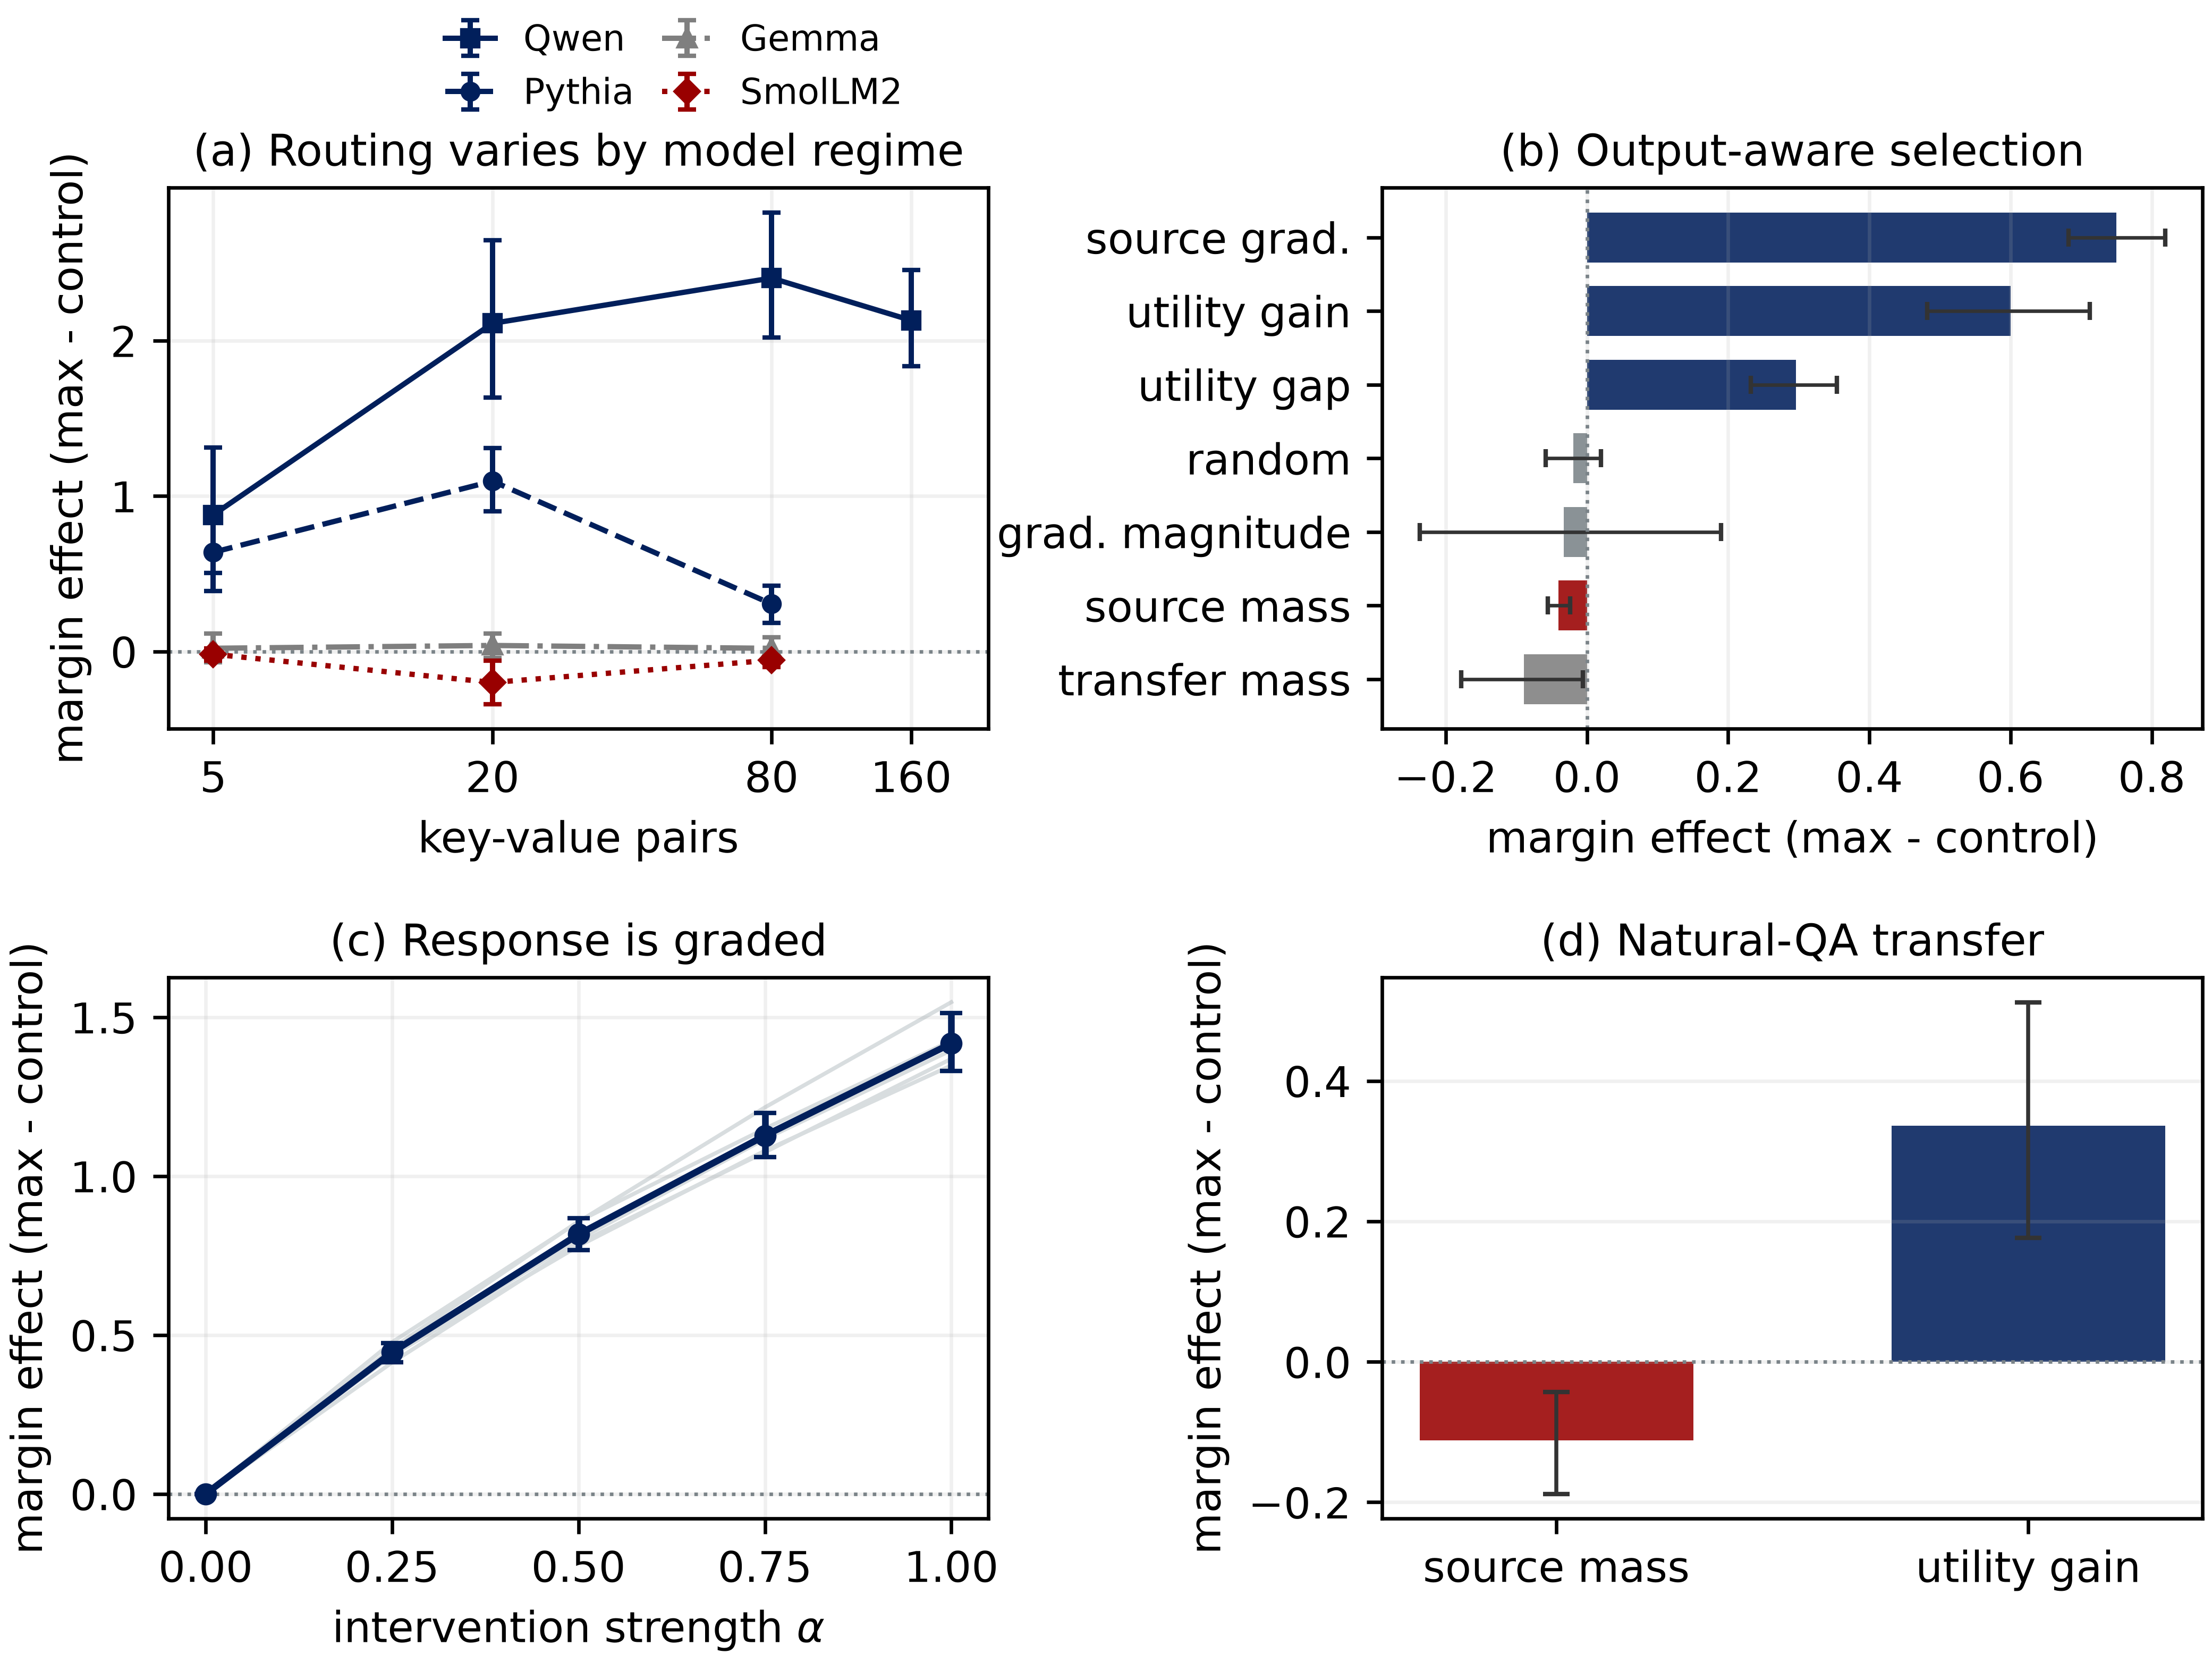
\includegraphics[width=0.85\textwidth]{figures/fig_pretrained_summary.png}
\caption{Fixed-spectrum routing transfers conditionally across pretrained models. Qwen and Pythia
are routing-responsive in the selected circuit, Gemma is saturated, and source-mass selection mismatches the useful SmolLM2 circuit
(a,b). The repaired effect is graded (c) and transfers to natural QA (d). Error bars show 95\% intervals;
faint lines in (c) are independent calibration seeds.}
\label{fig:pretrained-summary}
\end{figure*}

The pretrained models show why the utility term matters. Qwen and Pythia gain margin when source-max replaces
the distractor control. Gemma stays accurate as context grows and gains little from extra source mass, even
though source-min reliably harms it. This is the saturation regime predicted by Proposition~\ref{prop:utility}:
removing evidence matters, while extra routing has little left to add. A quantized Qwen2.5-7B run preserves
the positive margin direction.

SmolLM2 provides the complementary case. Its preregistered source-mass selector fails, yet ranking heads on
disjoint calibration examples by output-conditioned gradient or utility restores a positive effect. A ten-seed
ablation ranks source gradient, utility gain, and utility gap above source mass and transfer mass. Rankings vary
by architecture, but the broader lesson holds: circuit selection must account for the output.

Interpolating from the natural row to the utility-selected swap gives a monotone margin path over five
calibration seeds. On context-grounded natural QA, utility-selected routing improves margin over a
displacement-matched control, while source-mass selection harms it. Across six disjoint calibration seeds, the
utility-selected contrast is $+.378$ (hierarchical 95\% CI $[+.253,+.520]$; exact and Holm-adjusted
$p=.03125$). All competence gates pass. An unconstrained generation audit finds no first-answer or repetition
cost.

The selector results judge a selector by the frozen circuits it finds and their paired margin effects. They do
not test whether the per-row utility functional predicts a finite swap effect; the held-out predictor audit in
Table~\ref{tab:utility-replication} serves that separate purpose.

\begin{table*}[!t]
\centering
\scriptsize
\setlength{\tabcolsep}{1.8pt}
\begin{tabular*}{\textwidth}{@{\extracolsep{\fill}}llrlrrrrr}
\toprule
\multicolumn{2}{l}{\textbf{Fixed-spectrum assignment}} & $n$ & Units & Unpatched & $\Delta$ source-max & $\Delta$ source-min & $\Delta$ distractor & \textbf{max $-$ distractor} \\
\midrule
Single evidence & $\beta=1$ & 8,192 & Acc. & $.619$ & \helpful{$+.153$} & \harmful{$-.043$} & \neutral{$+.011$} & \helpful{$+.142$} \\
 & $\beta=4$ & 8,192 & Acc. & $.619$ & \helpful{$+.298$} & \harmful{$-.048$} & \neutral{$+.025$} & \helpful{$+.273$} \\
\midrule
Two evidence & $1\times$ & 2,048 & EM & $.952$ & \helpful{$+.019$} & \harmful{$-.559$} & \neutral{$+.012$} & \helpful{$+.007$} \\
 & $5\times$ & 2,048 & EM & $.484$ & \helpful{$+.066$} & \harmful{$-.291$} & \neutral{$+.023$} & \helpful{$+.043$} \\
\midrule
Pretrained KV & Pythia-1.4B & 384 & Margin & $-3.805$ & \helpful{$+.826$} & \harmful{$-1.022$} & \neutral{$+.146$} & \helpful{$+.680$} \\
 & Qwen2.5-1.5B & 512 & Margin & $-4.035$ & \helpful{$+2.044$} & \harmful{$-.758$} & \neutral{$+.162$} & \helpful{$+1.882$} \\
 & Qwen2.5-7B & 288 & Margin & $-3.361$ & \helpful{$+.623$} & \harmful{$-.907$} & \neutral{$+.055$} & \helpful{$+.568$} \\
 & Gemma-2-2B & 384 & Margin & $+2.234$ & \helpful{$+.040$} & \harmful{$-1.373$} & \neutral{$+.013$} & \helpful{$+.027$} \\
\midrule
\multicolumn{2}{l}{\textbf{Output-conditioned circuit selection}} & $n$ & Units & \multicolumn{2}{c}{$\Delta M$ versus matched control} & $\Delta M$ source mass & $\Pr(\Delta M>0)$ & \textbf{utility $-$ source} \\
\cmidrule(lr){5-6}
Task & Model & & & Utility gain & Utility gap & & & \\
\midrule
Pretrained KV & Pythia-1.4B & 384 & Margin & \helpful{$+.519$} & \helpful{$+.359$} & \neutral{$+.006$} & $.810$ & \helpful{$+.513$} \\
 & SmolLM2-1.7B & 384 & Margin & \helpful{$+1.253$} & \helpful{$+.859$} & \neutral{$+.006$} & $.969$ & \helpful{$+1.247$} \\
 & Qwen2.5-1.5B & 384 & Margin & \helpful{$+1.493$} & \helpful{$+1.493$} & \helpful{$+.069$} & $.956$ & \helpful{$+1.424$} \\
\bottomrule
\end{tabular*}
\caption{Benchmark summary. Units make upper-block baselines comparable only within task. The lower block has
no unpatched baseline: it evaluates selector quality using fixed-spectrum control effects, not per-row utility
prediction; Table~\ref{tab:utility-replication} evaluates that prediction.
$\Pr(\Delta M>0)$ is the fraction of paired evaluation examples with a positive utility-gain source-max
minus matched-control margin. Bold final columns remain identifiable in grayscale. Full cells and 95\%
intervals are in the supplement.}
\label{tab:evidence-summary}
\end{table*}

Clean-to-corrupt activation patching rescues $+.308$ margin but only $2.5$--$3.3\%$ of median corruption damage.
It restores selected-head outputs after source-value corruption, so its magnitude is not directly comparable
to reassignment on an unchanged input.

\subsection{Natural Context Marks the Scope Boundary}

\begin{figure*}[!t]
\centering
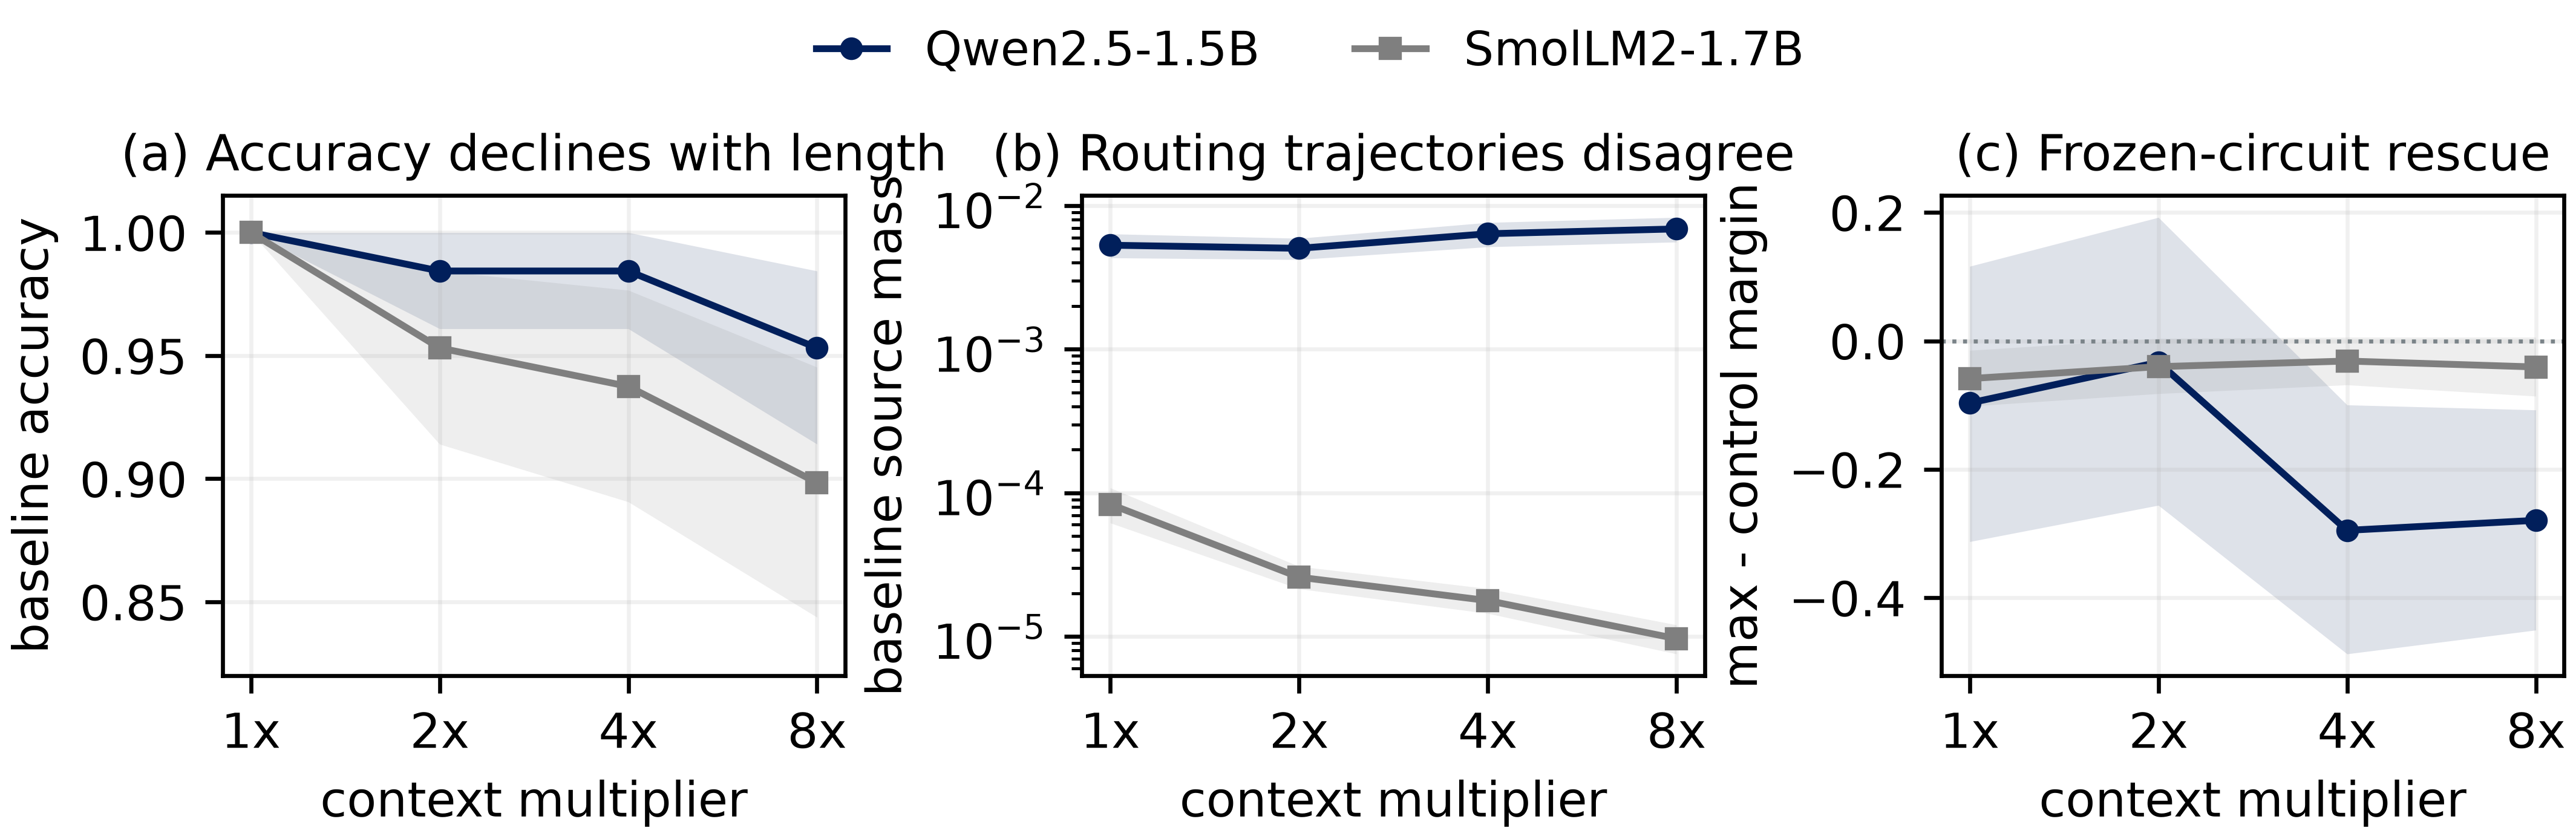
\includegraphics[width=0.76\textwidth]{figures/fig_natural_length_ladder.png}
\caption{Natural-QA degradation follows divergent routing trajectories. Circuits are frozen from four through
32 passages, shown as $1\times$--$8\times$ context. Accuracy falls (a), source routing moves in opposite
directions (b), and rescue stays flat or weakens (c). Bands are hierarchical 95\% intervals.}
\label{fig:natural-length-ladder}
\end{figure*}

The fixed-context natural-QA result establishes causal routing in ordinary text. The length ladder is a scope
test: it asks whether the same fixed-context protocol remains informative as context grows. We select the circuit
at four passages, freeze every choice, and append unrelated passages to form nested 4, 8, 16, and 32-passage
contexts. Hierarchical intervals resample calibration seeds and paired questions, so repeated observations from
one circuit are not treated as independent models.

Both Qwen and SmolLM2 lose margin and accuracy by 32 passages, yet their source-mass trajectories diverge.
Qwen source mass rises as intervention rescue weakens. SmolLM2 source mass falls while rescue stays flat.
The shared degradation therefore lies outside a single source-mass trajectory, which is the intended boundary
condition for this diagnosis rather than a failed prediction of it.

This result marks the boundary of the protocol. At a fixed context, a spectrum-preserving swap measures whether a
chosen circuit can use reassigned evidence. As contexts grow, representation quality, distractor semantics,
answer competition, and computation outside that circuit can also matter. The theorem therefore concerns a
specified swap at a fixed context, while the full set of long-context bottlenecks remains open. Exact
32-minus-4 changes and hierarchical intervals appear in the supplement.

The competence checks make the remaining boundary equally clear. In the arity study, the two-evidence task
passes and supports the mass-preserving control; the three-evidence interval includes zero, and the
four-evidence model misses competence. Higher arity remains unresolved. An eight-token generation audit also
leaves first-answer accuracy and repetition unchanged, so simple format collapse is not driving the result.

\subsection{Identification and Replication Audits}

We then ask whether the result depends on one calibration sample, patch budget, or model family. Across three
frozen Qwen calibration seeds, selected circuits are positive at every head budget. Adjacent-layer effects are
smaller and inconsistent, while random layers average near zero (Table~\ref{tab:selection-audit}).

\begin{table}[!t]
\centering
\small
\setlength{\tabcolsep}{4.0pt}
\begin{tabular}{lrrr}
\toprule
Circuit & Mean $\Delta M$ & Hierarchical 95\% CI & Seed SD \\
\midrule
Selected, $K=2$ & \helpful{+.460} & \helpful{[+.233,+.723]} & .180 \\
Selected, $K=4$ & \helpful{+1.054} & \helpful{[+.652,+1.493]} & .346 \\
Selected, $K=8$ & \helpful{+1.107} & \helpful{[+.739,+1.519]} & .293 \\
Adjacent $-1$ & \neutral{+.147} & \neutral{[-.002,+.332]} & .155 \\
Adjacent $+1$ & \neutral{-.131} & \neutral{[-.390,+.211]} & .323 \\
Random layer & \neutral{-.059} & \neutral{[-.207,+.101]} & .151 \\
\bottomrule
\end{tabular}
\caption{The selected Qwen circuit is stable across seeds and head budgets. Intervals resample
calibration seeds and paired examples; SD is across seedwise mean effects.}
\label{tab:selection-audit}
\end{table}

The utility relation also survives a separate replication check. Circuits are chosen by source mass on
disjoint calibration examples; utility is then computed on held-out evaluation rows. Across three seeds per
family, every competent source-max cell is positive, and predicted effects rank the exact effects within each
cell (Table~\ref{tab:utility-replication}). The approximation is imperfect at large effects, so we use it as a
local ranking signal rather than a calibrated finite-effect estimator. For the 32 controlled cell means in
Figure~\ref{fig:capacity-assignment}b, the actual-on-predicted fit is $1.387x-.102$ (Pearson $.978$), which
deviates from identity calibration.

\begin{table}[!t]
\centering
\small
\setlength{\tabcolsep}{4.0pt}
\begin{tabular}{lrrr}
\toprule
Model & Mean Spearman & Seed range & Sign agreement \\
\midrule
Qwen2.5-1.5B & \utilityhelpful{.866} & \utilityhelpful{[.832,.898]} & .805 \\
Pythia-1.4B & \utilityhelpful{.544} & \utilityhelpful{[.500,.586]} & .807 \\
Gemma-2-2B & \utilityhelpful{.554} & \utilityhelpful{[.534,.582]} & .714 \\
\bottomrule
\end{tabular}
\caption{Held-out local utility ranks exact source-max effects across pretrained families. Means and
ranges summarize three disjoint calibration seeds; calibration-error diagnostics appear in the supplement.}
\label{tab:utility-replication}
\end{table}

The exact Qwen rerun keeps precision, lengths, contrast, and sample counts fixed. All five new seeds are positive
(mean $+.042$); the combined six-seed test gives $p=.03125$, while the original $+1.882$ magnitude is atypical.

Output-conditioned selectors lead in each family, although their internal ranking changes by architecture.
Full selector results and competence-gate failures appear in the supplement.

\paragraph{Code availability.}
An anonymized code package with configurations, result artifacts, and analysis scripts accompanies the
supplementary release and will be made public on acceptance.

\section{Limitations}

\begin{itemize}
    \item Evidence positions must be identifiable. Source-max uses labels and serves as a causal probe; it is
    unsuitable as a deployable inference algorithm.
    \item Utility selection needs disjoint task-conditioned calibration and varies across model families.
    \item The reassignment is an off-manifold counterfactual. Endogenous rows show a positive conditional
    source-mass coefficient, but their closest-spectrum paired effect is inconclusive; the swap still identifies
    downstream sensitivity rather than the mechanism that produced the row.
    \item Higher evidence arity remains inconclusive or competence-limited; order-dependent computation is
    outside the current intervention.
    \item Natural long-context failure has multiple causes. We make no universal source-mass-loss claim.
\end{itemize}

\section{Conclusion}

Attention concentration tells us how much selectivity is available, while assignment tells us where that
selectivity goes. Our capacity--assignment decomposition and utility term identify when a fixed-spectrum swap
changes the target margin. This gives a local claim about the patched circuit.

The intervention reproduces across controlled retrieval, two-evidence computation, and pretrained models. Qwen and
Pythia respond to reassignment in the selected circuits, Gemma is saturated, and SmolLM2 benefits from
output-conditioned circuit selection. Dose response, disjoint calibration, layer controls, and seedwise
replication support these distinctions.

Natural QA carries the protocol into ordinary language at a fixed context. The length ladder then marks its
boundary: accuracy can decline even when source mass and intervention rescue follow different trajectories.
The protocol diagnoses a specified routing event and leaves the full account of long-context failure open.

{\small
\bibliography{references}
}

\end{document}
